\section{Kết quả}\label{sec:results}

Phần này trình bày kết quả theo hai mạch phân tích. \textbf{Mạch thứ nhất} (từ \S\ref{sec:start} đến~\ref{sec:denominator}) phân tích tác động tuần tự của ba phép kiểm soát lên hiệu quả hợp tác giữa các tác nhân. \textbf{Mạch thứ hai} (từ \S\ref{sec:termG} đến~\ref{sec:rl}) xác định giá trị còn lại thông qua ba thừa số $G$, $L$ và $\kappa$, và kết thúc bằng thảo luận về huấn luyện. Trừ khi ghi chú khác, các số liệu đều ở mức tin cậy A (\S\ref{sec:setup}); phạm vi đo của từng phép được ghi ngay tại bảng tương ứng. Bảng tra cứu ký hiệu ở Bảng~\ref{tab:cheatsheet}.

% ---------------------------------------------------------------
\subsection{Lợi ích của pipeline và mức dao động nền của phép đo}\label{sec:start}

\begin{table}[h]\centering\small
\begin{tabular}{@{}l c c c c@{}}
\toprule
Task & Solver 1 lượt & Pipeline \texttt{PSVA} & Chênh lệch & Hệ số token sinh\\
\midrule
GSM8K & 0,632 & \textbf{0,744} & $+11{,}2$ & $2{,}9\times$\\
MATH  & \textbf{0,405} & 0,345 & $-6{,}0$ & $6{,}63\times$\\
\bottomrule
\end{tabular}
\caption{So sánh pipeline đầy đủ bốn vai trò với một lần sinh duy nhất (Qwen-1.5B; đo một lần trên
toàn bộ tập). Hai cột giữa là độ chính xác, thang 0--1; cột \emph{Chênh lệch} tính bằng điểm phần trăm.}
\label{tab:pipeline}
\end{table}

Bảng~\ref{tab:pipeline} cho thấy kết quả trước khi áp dụng bất kỳ biện pháp kiểm soát nào. Trên GSM8K, pipeline hơn 11,2 điểm, trong khi trên MATH, nó tiêu tốn gấp 6,63 lần chi phí sinh token nhưng lại kém hơn 6 điểm. Cần lưu ý hai điểm quan trọng. \emph{Thứ nhất}, kiểm định thống kê dựa trên một đại lượng gần tương tự nhưng không hoàn toàn trùng khớp: qua 5 fold, hiệu số $\texttt{PSVA}-\texttt{PS} = +5{,}6$ điểm (KTC $[+3{,}3;+7{,}9]$; $t=6{,}89$) --- lợi ích trên GSM8K là có ý nghĩa thống kê. \emph{Thứ hai}, phép hiệu chuẩn mức dao động nền (\S\ref{sec:setup}) cho thấy hai phép đo trên 100 bài có thể chênh nhau tới 7 điểm; vì vậy, các hiệu ứng từ phép đo đơn lẻ chỉ được đọc như tín hiệu thăm dò.

Mục tiếp theo áp dụng phép kiểm soát thứ nhất: lợi ích này đến từ sự phối hợp giữa các vai trò hay chỉ đơn thuần là do số lượng lần sinh tăng lên?

% ---------------------------------------------------------------
\subsection{Giá trị nằm ở nhiều lần sinh độc lập hơn là ở cơ chế phối hợp}\label{sec:budget}

\begin{table}[h]\centering\small
\begin{tabular}{@{}l c c@{}}
\toprule
Bộ tổng hợp (cùng 8 lần sinh) & MATH 1.5B & MATH 7B\\
\midrule
\texttt{greedy} & 0,50 & \textbf{0,72}\\
\texttt{maj@8}     & 0,60 & \textbf{0,73}\\
\texttt{llm\_agg@8} & 0,41 & \textbf{0,47}\\
\texttt{oracle@8}      & 0,73 & \textbf{0,85}\\
\bottomrule
\end{tabular}
\caption{So sánh các bộ tổng hợp với cùng ngân sách 8 lần sinh (hàng trên cùng là mốc 1 lượt để tham chiếu). Các ô là độ chính xác, thang 0--1.}
\label{tab:budget}
\end{table}

Bảng~\ref{tab:budget} cố định ngân sách và chỉ thay đổi \emph{phương thức tổng hợp}. Từ đó rút ra bốn kết luận.

\emph{Thứ nhất}, bộ tổng hợp dùng LLM - \texttt{llm\_agg@8} kém hơn bỏ phiếu đa số - \texttt{maj@8} từ 19 đến 26 điểm ở cùng chi phí; ở model 7B, nó thậm chí còn kém cả \texttt{greedy} một lượt. Nó làm hỏng 21 câu trả lời đúng (với 1.5B) và 26 câu (với 7B), trong khi chỉ sửa được 2 và 0 câu sai. Phân tích 600 trace cho thấy 65\% số lần nó sao chép nguyên văn ứng viên \emph{cuối cùng} --- gần như một quy tắc dựa trên vị trí hơn là một bộ chọn dựa trên nội dung; 100\% lượt không sinh ra đáp án mới.

\emph{Thứ hai}, lợi ích của bỏ phiếu đa số giảm khi năng lực model nền tăng. Ở model 1.5B, \texttt{maj@8} cải thiện 10 điểm phần trăm, chiếm 43\% mức cải thiện tối đa lý thuyết 23 điểm phần trăm. Ở model 7B, mức cải thiện chỉ còn 1 điểm phần trăm, tương ứng 8\% trên mức tối đa 13 điểm phần trăm. Khoảng cách \texttt{oracle@8} - \texttt{maj@8} (13 và 12 điểm phần trăm) sẽ được dùng lại ở \S\ref{sec:kappa} như chặn trên cho mọi bộ chọn.

\emph{Thứ ba}, một đối chứng tách được ảnh hưởng của ``phối hợp'' khỏi ảnh hưởng của ``thêm lần sinh''. Khi cho giải lại mà \emph{không} xem phê bình của verifier, kết quả bằng đúng giải lại \emph{có} xem phê bình ($\texttt{rerun} = \texttt{loop}$, cùng cho $0{,}453$). Lợi ích vì vậy đến từ lần sinh thêm, không từ nội dung phản hồi. (Một phép đo đơn lẻ trước đó cho $+20$ điểm nhưng không tái lập: trên 5 fold chỉ còn $+4{,}0$ điểm.) Nhất quán với điều đó, biến thể vòng lặp giải-rồi-chấm --- rẻ hơn pipeline đủ vai trò --- còn thắng nó trên MATH: $+4{,}0$ điểm (KTC $[+0{,}5;+7{,}5]$; $t=3{,}21$) ở cùng chi phí.

\emph{Thứ tư}, phần ``gây hại'' của aggregator phần lớn là hiện vật đo lường. Chỉ 73--81\% lượt tổng hợp phát ra đáp án trong khung để chấm được; thêm một cơ chế dự phòng miễn phí (thiếu khung thì lấy đáp án của verifier, không gọi thêm model) đưa \texttt{A\_gain} trên MATH 1.5B từ $-6{,}4$ điểm lên $+0{,}8$ điểm. Một lần chạy khác (bộ bài khác, không lượng tử hoá) cho $+8{,}0$ điểm; sau khi vá lỗi định dạng, hai ước lượng cùng phía không âm, phần chênh còn lại quy cho khác bộ bài và khác độ chính xác số.\mucB

Sau phép kiểm soát chi phí, yếu tố chắc chắn có giá trị duy nhất là ``các lần sinh độc lập bổ sung''. Mục tiếp theo đặt câu hỏi: những lần sinh đó nên do vai trò nào và model cỡ nào đảm nhiệm?

% ---------------------------------------------------------------
\subsection{Phân rã đóng góp theo vai trò bằng giá trị Shapley}\label{sec:shapley}

Trước khi phân tích hành vi chi tiết, chúng tôi đo lường đóng góp của từng vai trò bằng giá trị Shapley \cite{shapley1953}: chạy đủ $2^4 = 16$ tổ hợp bật/tắt bốn vai trò (xem Hình~\ref{fig:shapleyfw}); đóng góp $\varphi_i$ của một vai trò là trung bình mức thay đổi độ chính xác khi thêm nó vào mọi tổ hợp con --- đây là cách phân bổ duy nhất thỏa mãn các tiên đề về hiệu quả, đối xứng và cộng tính.

\begin{figure}[t]\centering
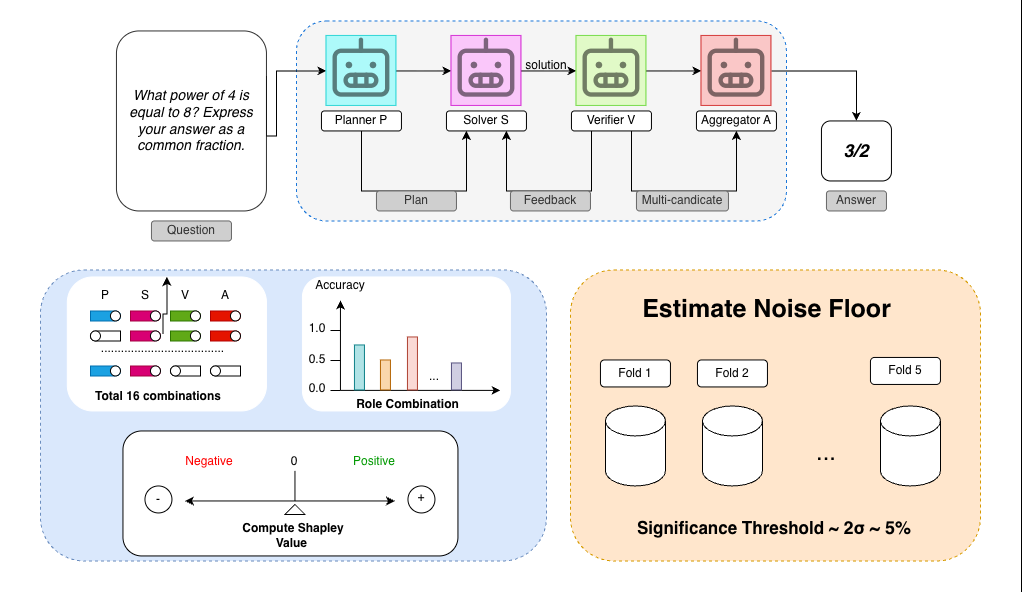
\includegraphics[width=0.9\linewidth]{figs/pipeline_shapley_overview.png}
\caption{Sơ đồ pipeline bốn vai trò, 16 tổ hợp bật/tắt để tính giá trị Shapley, và quy trình ước lượng nhiễu qua 5 fold.}
\label{fig:shapleyfw}
\end{figure}

\begin{table}[h]\centering\small
\begin{tabular}{@{}l c c@{}}
\toprule
Vai trò & GSM8K 1.5B ($N=1319$) & MATH-500 1.5B ($N=500$)\\
\midrule
Solver     & $+0{,}252$ $[+0{,}242;+0{,}263]$ & $+0{,}145$ $[+0{,}128;+0{,}161]$\\
Verifier   & $+0{,}252$ (đối xứng cấu trúc với Solver) & $+0{,}145$ (đối xứng)\\
Aggregator & $+0{,}190$ $[+0{,}182;+0{,}199]$ & $+0{,}150$ $[+0{,}134;+0{,}167]$\\
Planner    & $\mathbf{-0{,}014}$ $[-0{,}030;+0{,}002]$ & $+0{,}017$ $[-0{,}008;+0{,}043]$\\
\bottomrule
\end{tabular}
\caption{Giá trị Shapley của bốn vai trò, mọi vai trò đều 1.5B. Các giá trị $\varphi$ ở thang 0--1
(phần độ chính xác quy cho vai trò đó). KTC 95\% bootstrap theo câu hỏi --- \emph{không có fold},
nên đọc kèm mức dao động nền ở \S\ref{sec:setup}; trên MATH mọi chênh lệch giữa các vai trò đều dưới
mức dao động nền nên thứ hạng không có ý nghĩa.}
\label{tab:shapley}
\end{table}

Bảng~\ref{tab:shapley} cho thấy ba điểm chính. \emph{Thứ nhất}, Solver và Verifier chiếm phần lớn giá trị; Planner ở 1.5B có đóng góp âm trên GSM8K --- rõ nhất ở cặp tổ hợp: $SA = 0{,}682 \to PSA = 0{,}562$, việc thêm planner làm giảm 12 điểm. \emph{Thứ hai}, đóng góp thay đổi theo năng lực: khi nâng riêng planner lên 7B, $\varphi_P$ chuyển từ $-0{,}023$ lên $+0{,}055$ (chênh $+0{,}078$; KTC $[+0{,}049;+0{,}109]$) --- planner âm là hệ quả của model yếu, không phải bản chất vai trò. Nâng riêng verifier lên 7B đẩy $\varphi_V$ từ $+0{,}269$ lên $+0{,}462$ --- verifier là vai trò nhạy cảm nhất với năng lực, báo trước cho \S\ref{sec:roles}. \emph{Thứ ba}, chỉ số tương tác Shapley cho thấy $S$, $V$, $A$ thay thế lẫn nhau mạnh ($I \approx -0{,}21$ đến $-0{,}27$ ở cả hai task): ba vai trò này đang thực hiện các phiên bản của cùng một nhiệm vụ, chứ không bổ sung cho nhau.

Một giới hạn quan trọng của phép đo này: Shapley phân bổ giá trị cho \emph{nhãn vai trò}, không cho \emph{chức năng} --- nếu planner lén giải bài, công của nó vẫn được ghi cho nhãn ``Planner'' dù hành vi thực tế là của solver. Mục tiếp theo phân tích trace để trả lời liệu các vai trò có thực sự làm đúng chức năng của mình hay không.

% ---------------------------------------------------------------
\subsection{Khoảng cách giữa vai trò được gán và vai trò thực thi}\label{sec:roles}

Bảng~\ref{tab:behavior} tổng hợp hành vi từ trace, cho thấy sự chuyên biệt hoá vai trò phần lớn chỉ là hình thức ở model nhỏ: planner --- mặc dù bị cấm tính đáp án --- vẫn chứa đáp án đúng trong 34,7\% câu MATH (45,3\% trường hợp còn đưa ra cả khung đáp án); khi có plan, solver chỉ sao chép (độ dài trung vị lời giải là 19 ký tự, so với 664 khi không có plan). Ở model 7B, các hiện tượng này gần như biến mất --- nhưng ở mức năng lực đó, pipeline lại thua solver đơn lẻ. Trên 2.000 lượt ở cả bốn ô, aggregator chỉ 3 lần đưa ra một đáp án mới và đúng: vai trò tổng hợp không thực hiện tính toán ở mọi mức năng lực.

\begin{table}[h]\centering\small
\begin{tabular}{@{}l c c c c@{}}
\toprule
Chỉ số hành vi (trace) & GSM8K 1.5B & MATH 1.5B & GSM8K 7B & MATH 7B\\
\midrule
Planner rò rỉ đáp án đúng & 14,0\% & 34,7\% & 1,0\% & 4,0\%\\
Solver không sinh số mới & 60,7\% & 62,0\% & 1,0\% & 11,0\%\\
Độ dài lời giải solver & 19 & 344 & 821 & 1247\\
Verifier can thiệp & 32,7\% & 38,0\% & 4,0\% & 14,0\%\\
Aggregator lặp lại đáp án của verifier & 93,3\% & 73,3\% & 100\% & 97,0\%\\
\bottomrule
\end{tabular}
\caption{Hành vi theo từng ô (task $\times$ năng lực, với $n=100--150$ mỗi ô, đo trên trace).}
\label{tab:behavior}
\end{table}

Hai bằng chứng nhân quả hỗ trợ cho bảng này. \emph{Thứ nhất}: chỉ cần bỏ dòng cấm ``Do NOT compute the final answer'' khỏi prompt của planner, solver hạ nguồn \emph{tăng} $+3{,}8$ điểm trên MATH và $+3{,}3$ trên GSM8K --- hướng dẫn chỉ che giấu đáp án chứ không ngăn planner tính toán, và việc che giấu này lại gây hại. \emph{Thứ hai}, khi hoán vị prompt giữa các vị trí, độ chính xác không phân biệt được: trên GSM8K $0{,}660 = 0{,}660$ (cấu hình \texttt{solo} đạt $0{,}673$); trên MATH $\texttt{swap}-\texttt{normal} = +5{,}3$ điểm nhưng $t=1{,}84$, KTC $[-2{,}7;+13{,}4]$ --- không đạt ý nghĩa thống kê. Mặc dù KTC rộng không cho phép loại trừ hoàn toàn hiệu ứng cỡ vừa, chúng tôi chỉ ghi nhận rằng không có bằng chứng cho thấy ``danh tính vai trò'' ảnh hưởng đến kết quả.

Vai trò kiểm cũng không thực sự kiểm soát. Ba phép đo độc lập: (i) Khi can thiệp, verifier 1.5B đúng chỉ 56--59\% số lần --- gần như ngẫu nhiên; verifier 7B đúng 98\%. (ii) Thí nghiệm tiêm lỗi --- sửa kết quả một bước tính trong chuỗi lời giải vàng rồi hỏi model ``có lỗi tính toán không'' --- cho thấy 1.5B trả lời ``không có lỗi'' gần 100\% số bài, tức mù với lỗi đã tiêm; 7B vượt qua cổng hiệu lực và phân biệt được bài sạch với bài đã bị sửa ($+0{,}651$ trên tầng bài nó tự giải được; tầng nó \emph{không} tự giải được chỉ có $n=9$ nên câu hỏi ``kiểm có tách khỏi giải không'' còn bỏ ngỏ). (iii) Lưới \texttt{V\_gain} (Bảng~\ref{tab:vgaingrid}) cho thấy lượt kiểm chỉ sinh lợi trong một dải hẹp.

\begin{table}[h]\centering\small
\begin{tabular}{@{}l c c@{}}
\toprule
\texttt{V\_gain} (điểm; min--max theo fold) & GSM8K & MATH\\
\midrule
1.5B & $+4{,}4$ $[+1;+8]$, 5/5 dương & $+1{,}4$ $[-1;+4]$\\
7B   & $+1{,}0$ $[-3;+5]$ & $+4{,}4$ $[+2;+8]$, 5/5 dương\\
\bottomrule
\end{tabular}
\caption{\texttt{V\_gain} theo task $\times$ năng lực (5 fold mỗi ô). Xếp bốn ô theo độ chính xác
của solver --- $0{,}402$ (ngợp); $0{,}598$ (có lợi); $0{,}668$ (có lợi); $0{,}884$ (bão hoà) --- lượt
kiểm chỉ sinh lợi trong dải solver-accuracy $\approx 0{,}60$--$0{,}67$: dưới dải thì ngợp, trên dải
thì hết lỗi để sửa.}
\label{tab:vgaingrid}
\end{table}

Yếu tố tác động rõ ràng nhất là năng lực của model ở lượt kiểm tra. Cùng trên 300 bài MATH (5 fold $\times$ 60), Bảng~\ref{tab:verifier} cho thấy:

\begin{table}[h]\centering\small
\begin{tabular}{@{}l c c c@{}}
\toprule
Lượt kiểm & Hiệu ứng (điểm) & KTC 95\% (điểm) & Sửa : Phá\\
\midrule
\textbf{Verifier 7B} (solver 1.5B) & $\mathbf{+14{,}0}$ & $[+7{,}4;\,+20{,}6]$ & $43:1$\\
Verifier 1.5B (cùng cỡ) & $+3{,}0$ & KTC chứa 0 & $15:6$\\
Phần riêng do cỡ model lớn hơn & $+11{,}0$ & $[+3{,}9;\,+18{,}1]$ & ---\\
\bottomrule
\end{tabular}
\caption{Tác động bất đối xứng năng lực ở lượt kiểm trên MATH. ``Sửa : Phá'' = số bài sai được sửa thành đúng so với số bài đúng bị phá thành sai; verifier cùng cỡ phá 6 bài, trong khi verifier 7B chỉ phá 1 bài trên cùng 300 bài.}
\label{tab:verifier}
\end{table}

Cơ chế từ trace: khi verifier can thiệp, nó tái sử dụng số liệu trung gian của solver với tỷ lệ thấp hơn khoảng 5 lần so với khi đồng ý ($0{,}20$--$0{,}23$ so với $0{,}96$). Vì vậy, hành vi can thiệp gần với giải lại hơn là kiểm tra từng bước; về tác động, lượt kiểm tương đương với một lần sinh bổ sung. Điều này phù hợp với giả thuyết rằng $+14{,}0$ điểm chủ yếu đến từ việc thêm một lần sinh của model mạnh hơn. Sự nhất quán cũng thể hiện ở chỗ: \texttt{V\_gain} có ý nghĩa trên MATH 7B ($+4{,}4$ điểm; KTC $[+1{,}5;+7{,}3]$) nhưng không có ý nghĩa trên MATH 1.5B ($+1{,}4$; $p=0{,}235$). Lưu ý cho \S\ref{sec:protocols}: verifier \emph{sinh ra chuỗi mới}, nên thuộc lớp sửa chữa --- $L$ của nó đo được là $1/300 \approx 0{,}003$, rất nhỏ nhưng không phải bằng 0 về cấu trúc.

Con số $+14{,}0$ đang so với model yếu. Mục tiếp theo áp dụng phép kiểm soát thứ hai và thứ nhất đồng thời: so sánh với mốc model mạnh và xét đến chi phí token.

% ---------------------------------------------------------------
\subsection{Model mạnh đơn lẻ vẫn là mốc chuẩn về hiệu quả và chi phí}\label{sec:baseline}

\begin{table}[h]\centering\small
\begin{tabular}{@{}l c c c c@{}}
\toprule
Cấu hình & GSM8K & MATH & Token 7B (GSM8K) & Token 7B (MATH)\\
\midrule
S1.5B + V7B & 0,810 & 0,563 & 105k & 119k\\
\textbf{S7B đơn lẻ} & \textbf{0,910} & 0,593 & 120k & 152k\\
S7B + V7B & 0,900 & \textbf{0,670} & 205k & 261k\\
\bottomrule
\end{tabular}
\caption{So sánh với mốc model mạnh: các cấu hình có lượt kiểm so với model mạnh chạy đơn lẻ (5 fold). Cột token chỉ tính token do model 7B sinh --- không thể so sánh trực tiếp giữa các cấu hình có cỡ model khác nhau; hiệu chỉnh được trình bày ở Bảng~\ref{tab:flop}. Hai cột giữa là độ chính xác (thang 0--1), hai cột cuối là số token (nghìn).}
\label{tab:baseline}
\end{table}

Bảng~\ref{tab:baseline} thay đổi mốc so sánh từ ``model yếu'' sang ``model mạnh đơn lẻ'', và bức tranh thay đổi. Cấu hình bất đối xứng S1.5B+V7B --- chính là cấu hình cho $+14{,}0$ điểm ở Bảng~\ref{tab:verifier} --- \emph{kém hơn} S7B đơn lẻ 10 điểm trên GSM8K và chỉ ngang bằng trên MATH. Cột chi phí cần hai hiệu chỉnh: (a) cột token gốc bỏ qua token của solver 1.5B; (b) token 7B đắt hơn token 1.5B khoảng 4,7--4,9 lần theo FLOP. Bảng~\ref{tab:flop} hiệu chỉnh về thang FLOP:

\begin{table}[h]\centering\small
\begin{tabular}{@{}l c c@{}}
\toprule
Tỷ số chi phí (bất đối xứng / S7B) & Token thô 7B & Trọng số FLOP\\
\midrule
GSM8K & $0{,}88\times$ (``rẻ hơn 12\%'') & $\mathbf{1{,}00\text{--}1{,}05\times}$ \\
MATH & $0{,}78\times$ (``rẻ hơn 22\%'') & $\mathbf{0{,}92\text{--}0{,}96\times}$ \\
\bottomrule
\end{tabular}
\caption{Hiệu chỉnh đơn giá token (độ nhạy ký tự/token quét 3,0--4,0). Chưa tính phần prefill --- model 7B phải \emph{đọc} bài làm của 1.5B --- nên hiệu chỉnh vẫn thiên vị cho cấu hình bất đối xứng.}
\label{tab:flop}
\end{table}

Kết luận: trên GSM8K, cấu hình bất đối xứng bị chi phối hoàn toàn (kém 10 điểm, chi phí FLOP tương đương); trên MATH, nó tiết kiệm biên 4--8\% với độ chính xác tương đương. Model mạnh đơn lẻ nằm trên đường Pareto ở cả hai task.

Điểm sáng duy nhất có ý nghĩa thống kê trong Bảng~\ref{tab:baseline} lại nằm ở cấu hình cùng cỡ: thêm V7B vào S7B trên MATH cho $+7{,}7$ điểm ($p=0{,}0075$; McNemar), với chi phí $1{,}7\times$ token. Theo ký hiệu ở \S\ref{sec:identity}, đây là trường hợp $\acc(E) > \acc(I)$ --- và đáng chú ý, nó xảy ra ở \emph{chênh lệch bằng 0}. Cùng cấu hình trên GSM8K lại cho $1{,}7\times$ chi phí để mất 1 điểm --- lợi ích của lượt kiểm cùng cỡ phụ thuộc vào task. Chúng tôi sẽ quay lại điểm dữ liệu này ở \S\ref{sec:termG}, nơi nó là điểm duy nhất ủng hộ cho nửa dương của quy luật chênh lệch.

Vì cùng một cặp model trên cùng một họ bài xuất hiện với nhiều giá trị khác nhau trong báo cáo, Bảng~\ref{tab:doichieu} đối chiếu để tránh nhầm lẫn:

\begin{table}[h]\centering\small
\begin{tabular}{@{}l l l l l@{}}
\toprule
Con số & Đại lượng & Mốc so sánh & Thiết lập & Mục\\
\midrule
$+14{,}0$ điểm & hiệu ứng lượt kiểm & model yếu (\texttt{PS}) & prompt kiểm, 300 bài & \S\ref{sec:roles}\\
$-3{,}0$ điểm & độ chính xác cấu hình & model mạnh (S7B) & như trên, 5 fold & \S\ref{sec:baseline}\\
$-12{,}4$ điểm & $\dhonest = \acc(E)-\acc(I)$ & model mạnh & prompt \emph{giải}, kèm artifact, $n=500$ & \S\ref{sec:termL}\\
$-16{,}6$ điểm & $\dceil$ (trần lý tưởng) & model mạnh & prompt sửa, bootstrap & \S\ref{sec:transfer}\\
\bottomrule
\end{tabular}
\caption{Cùng cặp 1.5B$\to$7B trên miền toán, bốn đại lượng khác nhau. Sự khác dấu giữa dòng đầu và ba dòng sau phản ánh chính hiện tượng trung tâm: thay đổi mốc so sánh sẽ thay đổi dấu của hiệu ứng.}
\label{tab:doichieu}
\end{table}

Còn một phép kiểm soát chưa áp dụng: mẫu số. Mọi con số trên đều là trung bình toàn tập --- bao gồm cả những câu mà không có cơ chế nào cứu được.

% ---------------------------------------------------------------
\subsection{Kiểm soát mẫu số: phần lớn số câu vốn bất động}\label{sec:denominator}

\begin{table}[h]\centering\small
\begin{tabular}{@{}l c c c c@{}}
\toprule
Số lượt đúng /5 & $n$ & Solver & maj@5 & $\Delta$ (điểm)\\
\midrule
0/5 --- quá khó & 48 (32\%) & 0,000 & 0,000 & 0\\
1/5 & 20 (13\%) & 0,000 & 0,000 & 0\\
2/5 & 15 & 0,333 & 0,600 & $+26{,}7$\\
3/5 & 12 & 0,583 & 1,000 & $+41{,}7$\\
4/5 & 18 & 0,722 & 1,000 & $+27{,}8$\\
5/5 --- quá dễ & 37 (25\%) & 1,000 & 1,000 & 0\\
\bottomrule
\end{tabular}
\caption{Phân tầng theo số lần đúng trong 5 lần sinh (MATH 1.5B, $n=150$). Cột $\Delta$ là chênh lệch độ chính xác giữa \texttt{maj@5} và Solver.}
\label{tab:strata}
\end{table}

Bảng~\ref{tab:strata} phân 150 bài theo ``pool chứa bao nhiêu lời giải đúng''. Hai con số bất động cần phân biệt: theo cấu trúc pool, 57\% số câu (0/5 và 5/5) không thể có hiệu ứng với bất kỳ bộ tổng hợp nào --- không có gì để chọn hoặc không có gì để cải thiện; đối với bỏ phiếu đa số nói riêng, thêm tầng 1/5 (một phiếu không thắng nổi đa số) đưa tổng lên 70\%. Trên tầng khả tác động, hiệu ứng của bỏ phiếu là $+21{,}5$ điểm (các tầng 1--4/5) hay $+31{,}1$ điểm (tầng 2--4/5); trung bình toàn tập pha loãng còn $+9{,}3$ --- tỷ lệ pha loãng 2,3--3,3 lần tuỳ cách nhóm (tầng được xác định hậu nghiệm bằng chính kết quả sinh, nên đây là công cụ diễn giải, không phải mốc triển khai được). Một can thiệp $+10$ điểm thật chỉ tác động được tầng 2--4/5 (30\% số bài) sẽ hiện ra $+3{,}0$ điểm toàn tập --- dưới mức dao động nền.

Ba phép kiểm soát vậy là ngược chiều nhau: thiếu mẫu số $\Rightarrow$ đánh giá thấp; thiếu chi phí hoặc mốc $\Rightarrow$ đánh giá cao. Hạn chế tự khai: các hiệu ứng chủ lực ở \S\ref{sec:roles}--\ref{sec:baseline} chưa được phân tầng lại theo cách này (thiếu dữ liệu theo-bài cho từng tầng); con số toàn tập của chúng vì vậy là ước lượng thấp của hiệu ứng trên tầng khả tác động.

\emph{Hết mạch thứ nhất.} Bức tranh sau ba phép kiểm soát: giá trị dương chắc chắn duy nhất là lần sinh thêm; cấu hình sửa-bài-của-nhau thua model mạnh đơn lẻ. Hồi II xác định giá trị mất đi đâu và có quy luật nào đoán trước được hay không.

% ---------------------------------------------------------------
\subsection{Số hạng $G$: cơ hội co lại khi chênh lệch tăng}\label{sec:termG}

Quan sát thô trên 7 cặp model gộp nhiều lần chạy cho thấy: các cặp khác họ có cơ hội $G$ cao hơn khoảng 24\% (0,0597 so với 0,0481), nhưng các cặp khác họ cũng có chênh lệch năng lực nhỏ hơn (0,130 so với 0,167); hai biến này bị trộn hoàn toàn. Thiết kế tách biệt (tiền đăng ký) sử dụng 6 model, 15 cặp có hướng, trên cùng 499 bài MBPP, hồi quy
\begin{align*}
G &= \beta_0 + \beta_1\cdot\text{chênh} + \beta_2\cdot\text{khác\_họ}\\
\beta_1 &= -0{,}1922\ (p \approx 0)\\
\beta_2 &= +0{,}0045\ (\text{KTC } [-0{,}0051;+0{,}0140];\ p = 0{,}31).
\end{align*}
$R^2$ chỉ với chênh lệch là 0,824. KTC của $\beta_2$ nằm trọn dưới ngưỡng tương đương $+0{,}02$ đã khoá trước, cho thấy một kết quả null có thông tin: khác họ là tương quan giả; biến giải thích chính là chênh lệch năng lực. Dấu của $\beta_1$ đáng chú ý: chênh lệch càng lớn, cơ hội $G$ càng nhỏ --- model yếu càng đuối thì càng hiếm bài nó cứu được model mạnh. (Kết quả đa dạng pool --- 3 model cho 2,70/3 ứng viên phân biệt so với 1,91/3 khi cùng model --- chỉ được ghi là khác model; đối chứng khác-model-cùng-họ chưa chạy.)

Thêm nhánh sửa cho cả 15 cặp (tiền đăng ký) cho quy luật của trần:
\begin{equation}\label{eq:rule}
\dceil = +0{,}0218 - 0{,}2392 \times \text{chênh};\qquad R^2 = 0{,}60;\ p = 10^{-5};\
g^\ast \approx 0{,}09,
\end{equation}
trong đó $g^\ast = \beta_0/|\beta_1|$ là mức chênh nơi đường khớp cắt 0 (tức $\approx 9$ điểm accuracy; chúng tôi chưa ước lượng KTC cho $g^\ast$ nên nó là mô tả xu hướng, chưa phải quy tắc vận hành). Đẳng thức~\eqref{eq:identity} khớp 15/15 cặp. Đọc kèm bắt buộc: 0/15 cặp dương có ý nghĩa, 3/15 âm có ý nghĩa --- trên MBPP quy luật chỉ phát biểu được chiều phủ định (chênh vượt $\sim$0,09 thì giao thức sửa cho hiệu ứng âm); xác lập vùng dương cần cỡ 8 lần dữ liệu MBPP. Hai điểm dữ liệu ngoài MBPP soi vào nửa dương: cặp 7B$\to$14B trên MATH (chênh $0{,}044 < g^\ast$) đo được $-1{,}4$ điểm, KTC chứa cả hai phía, nên không ủng hộ; cấu hình cùng cỡ (chênh $=0$) trên MATH đo được $+7{,}7$ điểm có ý nghĩa (\S\ref{sec:baseline}), ủng hộ. Nửa dương vì vậy dừng ở mức "một điểm thuận, một điểm không kết luận". Chênh giải thích 82\% phương sai của $G$ nhưng chỉ 35\% của $L$; phần lớn biến thiên của thiệt hại đến từ yếu tố khác chưa định danh (đưa vào Hạn chế). (Ghi chú cơ chế\mucB: ngưỡng bảo toàn mà lượt sửa phải vượt tăng theo chênh nhanh gấp đôi khả năng bảo toàn thực của nó --- hệ số 2,18 so với 1,10; $p=0{,}0066$ --- gợi ý hiệu ứng âm phát sinh từ cấu trúc ngân sách $G$--$L$, không từ suy giảm năng lực nội tại của model mạnh.)

% ---------------------------------------------------------------
\subsection{Khả năng chuyển miền của quy luật}\label{sec:transfer}

Chúng tôi sử dụng đường khớp~\eqref{eq:rule} ước lượng trên MBPP để dự báo $\dceil$ trên MATH (tiền đăng ký; 3 cặp Qwen; KTC bootstrap ghép cặp 10\,000 lần). Kết quả được trình bày trong Bảng~\ref{tab:transfer}.

\begin{table}[htbp]
\centering
\small
\begin{tabular}{@{}l c c c c l@{}}
\toprule
Cặp & Chênh & $\dceil$ đo được & KTC 95\% & Dự báo từ MBPP & Kết luận\\
\midrule
7B$\to$14B & 0,044 & $-0{,}0140$ & $[-0{,}046;\,+0{,}018]$ & $+0{,}0108$ & nằm trong khoảng\\
1.5B$\to$7B & 0,244 & $-0{,}1660$ & $[-0{,}208;\,-0{,}124]$ & $-0{,}0361$ & ngoài khoảng\\
1.5B$\to$14B & 0,288 & $-0{,}0680$ & $[-0{,}102;\,-0{,}034]$ & $-0{,}0471$ & nằm trong khoảng\\
\bottomrule
\end{tabular}
\caption{Kiểm tra khả năng chuyển miền của quy luật chênh lệch (thang 0--1). Cột $\dceil$ đo được và dự báo có đơn vị điểm chính xác.}
\label{tab:transfer}
\end{table}

Hai trong ba dự báo nằm trong khoảng tin cậy 95\%, do đó quy luật không bị bác bỏ. Tuy nhiên, khoảng tin cậy khá rộng (0,064--0,084) nên phép kiểm có độ phân giải thấp. Hơn nữa, thứ tự ba điểm không đơn điệu (chênh 0,244 cho hiệu ứng âm sâu hơn chênh 0,288), vì vậy tính đơn điệu của quy luật chưa được xác nhận trên miền toán. Cặp 1.5B$\to$7B nằm ngoài một cách hệ thống, với $L = 0{,}208$, gấp khoảng 11 lần $G$. Hiện tượng này tái lập trong một phép đo độc lập trên cùng cặp ($-0{,}1380 \to -0{,}1660$). Như vậy, quy luật chỉ mô tả xu hướng chung; ngoại lệ xuất hiện khi model yếu quá kém so với độ khó của bài toán.

\subsection{Số hạng $L$: hình phạt của nội dung sai và vai trò ống dẫn của giao thức sửa}\label{sec:termL}

Đây là thí nghiệm chính của khảo sát (tiền đăng ký; chọn MATH-500 để đổi miền so với quan sát thăm dò gốc trên MBPP). Thiết kế được mô tả trong Hình~\ref{fig:exposure}: hai nhánh $I$ và $E$ dùng cùng một lệnh giải, chỉ khác nhau ở việc ngữ cảnh có kèm artifact của $W$ hay không. Kết quả được phân tầng theo nội dung artifact và trình bày trong Bảng~\ref{tab:exposure}.

\begin{table}[htbp]
\centering
\small
\begin{tabular}{@{}l c c c@{}}
\toprule
Tầng & MBPP 11--510\mucB & MBPP 511--974\mucB & MATH-500 (mức A)\\
\midrule
artifact sai  & $-19{,}0$ & $-19{,}3$ & $-27{,}2$ ($p\approx 0$; $n=261$)\\
artifact đúng & $+6{,}4$ & $+2{,}5$ & $+3{,}8$ ($p=0{,}012$; $n=239$)\\
\bottomrule
\end{tabular}
\caption{Hiệu ứng tiếp xúc $\acc(E)-\acc(I)$ (đơn vị: điểm phần trăm), phân tầng theo nội dung artifact. Hai cột MBPP là phân tầng hậu nghiệm (mức B); cột MATH là thí nghiệm tiền đăng ký (mức A).}
\label{tab:exposure}
\end{table}

Trên tầng artifact sai, độ chính xác của model mạnh giảm từ 46,4\% xuống 19,2\% --- ngay trên những bài mà nó vốn giải được gần một nửa. Ngược lại, artifact đúng giúp cải thiện độ chính xác. Tổng hợp trọng số của hai tầng tái tạo đúng $\dhonest = -12{,}4$ điểm. Kết luận về cơ chế: $D$ không phải là hình phạt của việc nhìn thấy artifact nói chung, mà là của việc nhìn thấy nội dung sai. Vì thiết kế không có lệnh sửa, chỉ riêng sự hiện diện của nội dung sai trong ngữ cảnh đã đủ tạo hiệu ứng âm. (Đối chứng cùng thiết lập cho ảnh hưởng thuần của độ dài ngữ cảnh chưa được thực hiện; đối chứng gần nhất --- chèn bối cảnh vô quan trong thiết lập kiểm\mucB{} --- cho $-3{,}6$ điểm, tức nhiễu ngữ cảnh thuần có hại nhẹ, nhỏ hơn hình phạt nội dung sai từ 7 đến 8 lần.) Quan sát này khớp với mức tái sử dụng thấp khi can thiệp ở \S\ref{sec:roles}: model mạnh ít sao chép bề mặt nội dung sai, nhưng vẫn bị nó neo hướng giải --- ảnh hưởng đi qua định hướng nhiều hơn qua trích dẫn.

Bảng~\ref{tab:222} chấm lại toàn bộ 500 bài theo cặp trạng thái ($W$ đúng/sai) $\times$ ($I$ đúng/sai), đồng thời ghi tỷ lệ $E$ đúng trong từng ô, nhằm trả lời câu hỏi khi model mạnh sai thì việc sửa có giúp ích hay không.

\begin{table}[htbp]
\centering
\small
\begin{tabular}{@{}l c c@{}}
\toprule
Tầng & $n$ & Tỷ lệ $E$ đúng (\%) \\
\midrule
$W$ đúng, $I$ đúng & 228 & 99,6\\
$W$ đúng, $I$ sai & 11 & 90,9\\
$W$ sai, $I$ đúng (vùng rủi ro) & 121 & 36,4 \quad (phá 63,6\%)\\
Cả hai sai & 140 & 4,3\\
\bottomrule
\end{tabular}
\caption{Phân tầng $2\times 2$ theo trạng thái của $W$ và $I$ trên MATH ($n=500$), kèm tỷ lệ $E$ đúng trong mỗi tầng.}
\label{tab:222}
\end{table}

Từ Bảng~\ref{tab:222} rút ra ba nhận xét chính. Thứ nhất, giao thức sửa đóng vai trò như một ống dẫn, không phải bộ sửa lỗi: gần như không tạo ra lời giải mới khi cả hai model đều trượt (4,3\% = 6/140), phá hủy ở quy mô lớn trên vùng rủi ro (63,6\% = 77/121), và truyền lại đáp án đúng của $W$ khi có (10/11 bài --- tầng quá nhỏ để ước lượng chặt chẽ). Thứ hai, ở cặp này tầng khai thác được nhỏ hơn vùng rủi ro 11 lần (11 so với 121 bài); tỷ lệ này co giãn theo chênh lệch, nhưng chưa được đo ở các mức chênh khác. Thứ ba, chiến lược “$W$ đúng thì giữ $W$” tương đương với oracle $\CEIL$. Ngay cả khi được cung cấp oracle này, mức tăng cũng chỉ là $+0{,}4$ điểm (đúng thêm 2/500 bài), vì $E$ vốn đã giữ được 99,6\% và 90,9\% trong hai tầng tương ứng. Kể cả với $\CEIL = 0{,}578$, giá trị này vẫn thấp hơn $I = 0{,}698$. Trong lớp giao thức sửa bất đối xứng đã đo, không có cấu hình nào đạt $\acc(E) > \acc(I)$ (0/15 cặp MBPP, tốt nhất $-3{,}0$ điểm; các cặp MATH trong Bảng~\ref{tab:transfer}); trường hợp $E>I$ duy nhất là cấu hình cùng cỡ ở \S\ref{sec:baseline}. Vấn đề không nằm ở việc “quên giữ $W$”, mà là $E$ phá vùng rủi ro. Trong các phương án đã thử (hai cổng oracle ở \S\ref{sec:kappa}), chỉ có việc không đưa artifact vào ngữ cảnh mới bảo vệ được vùng đó.

\subsection{Khả năng khai thác $\kappa$ và định tuyến: tín hiệu chắc chắn đạt chặn trên, tín hiệu học được không đạt}\label{sec:kappa}

\paragraph{Tín hiệu chắc chắn.}
Trên HumanEval, cùng model, cùng 4 lần sinh, chỉ khác nhau ở nguồn kiểm tra, kết quả được trình bày trong Bảng~\ref{tab:exec}.

\begin{table}[htbp]
\centering
\small
\begin{tabular}{@{}l c c c c c@{}}
\toprule
Điều kiện & greedy & exec3 & llm3 & exec3 phá & llm3 phá\\
\midrule
HE 1.5B  & 0,5375 & 0,6000 & 0,4812 & 0,0 & 2,8\\
HE 1.5B    & 0,5625 & 0,6438 & 0,4375 & 0,0 & 4,6\\
HE 7B      & 0,8000 & 0,8812 & 0,7812 & 0,0 & 2,6\\
HE 7B   & 0,7938 & 0,9000 & 0,7438 & 0,0 & 3,2\\
\bottomrule
\end{tabular}
\caption{So sánh chọn bằng chạy test (\texttt{exec3}) và LLM tự duyệt (\texttt{llm3}). Bốn hàng tương ứng với bốn điều kiện (hai model $\times$ hai hệ phần cứng); độ trôi phần cứng khoảng 0,03, nhỏ hơn hiệu ứng quan tâm nên kết luận về dấu vẫn đứng. Cột “phá” là số bài bị phá trên mỗi fold. }
\label{tab:exec}
\end{table}

exec3 không phá hủy bài nào trong cả 20/20 fold và đạt đúng \texttt{oracle@4} ở hai ô có ghi số (0,6438 và 0,8812). Ngược lại, llm3 phá hủy thì ở tất cả 20 fold. Mốc trung thực là greedy; bỏ phiếu đa số có hại trên code ($-11{,}3$ và $-13{,}1$ điểm) vì lời giải dài hiếm khi trùng nhau nguyên văn. Chênh lệch $exec3-\text{greedy}$ dao động từ $+6{,}3$ đến $+10{,}6$ điểm qua bốn điều kiện. Một điều kiện áp dụng quan trọng: khi model nền bão hòa (GSM8K 7B, solver 0,916), một bộ kiểm thực thi có độ chính xác 0,837 vẫn cho hiệu ứng ròng âm (26 phá / 6 sửa). Do đó, “có bộ kiểm chắc chắn” chỉ có giá trị khi còn tiềm năng cải thiện cải thiện.

\paragraph{Tín hiệu học được.}
Bộ phân loại được huấn luyện trên lỗi tiêm (lấy lời giải đúng rồi đổi một chữ số trong đáp án) và sau đó được dùng để phát hiện lỗi thật. Đây cũng chính là phép thử “thay một số trong đáp án, verifier có thấy không”. Kết quả được trình bày trong Bảng~\ref{tab:clf}.

\begin{table}[htbp]
\centering
\small
\begin{tabular}{@{}l c c c c@{}}
\toprule
Model & Tách biệt trên lỗi tiêm & Tách biệt trên lỗi thật & AUC & $\Delta$ độ chính xác\\
\midrule
1.5B & $-0{,}012$ & $+0{,}195$ & 0,528 & $-0{,}8$ điểm (1/5 fold dương)\\
\textbf{7B} & $\mathbf{+0{,}573}$ & $\mathbf{+0{,}693}$ & \textbf{0,893} & $\mathbf{+2{,}4}$ điểm (2/5 fold dương)\\
\bottomrule
\end{tabular}
\caption{Hiệu quả của bộ phân loại lỗi học được. Hai cột đầu là mức tách biệt điểm phân loại
giữa lời giải đúng và sai, đo trên lỗi tiêm và lỗi thật \todoTD{xác nhận định nghĩa chính xác
của đại lượng hai cột này}. Ở 1.5B, AUC $0{,}528 \approx$ đoán ngẫu nhiên: thay một chữ số trong
đáp án, verifier 1.5B không phát hiện được.}
\label{tab:clf}
\end{table}

Ở model 7B, tín hiệu đo được rất tốt (AUC = 0,893; trên lỗi thật còn tách tốt hơn lỗi tiêm, cần loại trừ khả năng bộ phân loại bắt đặc trưng bề mặt như độ dài; đối chứng chưa được thực hiện). Tuy nhiên, khi sử dụng tín hiệu này để chọn, mức cải thiện chỉ là $+2{,}4$ điểm, và chỉ 2/5 fold dương. Theo phép thử dấu của chính chúng tôi, mức tăng này chưa phân biệt được với 0. Như vậy, tín hiệu đo được không tự động trở thành tín hiệu dùng được; điều này củng cố phát biểu chặn trên dưới đây.

\paragraph{Phát biểu hợp nhất.}
Đặt cạnh nhau: trên code, khoảng cách $\texttt{oracle@}k-\texttt{maj@}k$ là $+21{,}3$ điểm và exec3 lấy gần trọn (đạt đúng \texttt{oracle@4}, phá 0 lần); trên toán, khoảng cách là 12--13 điểm (Bảng~\ref{tab:budget}) nhưng tín hiệu học được tốt nhất chỉ lấy $+2{,}4$ điểm.

\begin{quote}
Khoảng cách $\texttt{oracle@}k - \texttt{maj@}k$ là chặn trên cho giá trị của mọi bộ kiểm trên cùng pool. Tín hiệu chắc chắn (chạy test) lấy gần trọn chặn đó; tín hiệu học được trong khảo sát của chúng tôi chỉ lấy được một phần nhỏ, dù chất lượng đo lỗi rất cao. Nút thắt của miền toán vì vậy mang tính kép: vừa thiếu tín hiệu chắc chắn, vừa nghèo pool. Trong số bài mà \texttt{maj@5} sai, 71\% (48/68, tính từ Bảng~\ref{tab:strata}) là bài pool không chứa nổi một ứng viên đúng, tức không bộ chọn nào có thể cứu được.
\end{quote}

\paragraph{Định tuyến.}
Hai kết quả về “chọn lúc nào cần gọi thêm” đều ở mức B (đo một lần, $n=300$). Bộ định tuyến đồng thuận (chạy $S$ và $V$, chỉ gọi $A$ khi hai vai trò bất đồng) trên GSM8K giữ gần trọn phần lợi của pipeline với 77\% chi phí (0,720 so với 0,723 ở 2,32 so với 3 lượt); trên MATH đạt 0,413, bằng với solver đơn lẻ và không mang lại lợi ích. Cơ chế phía sau nhất quán với \S\ref{sec:termL}: tỷ lệ bài model yếu sai (tức tỷ lệ artifact sai trong ngữ cảnh) khoảng 33\% trên GSM8K so với 59\% trên MATH; khi hai vai trò bất đồng, $A$ cứu được 45,4\% trường hợp trên GSM8K nhưng chỉ 25,0\% trên MATH. Do đó, quan sát “định tuyến tiết kiệm ở đúng nơi ít cần tiết kiệm nhất” chỉ dừng ở mức B.

Hai trần cho cổng tiếp xúc (tính trên dữ liệu \S\ref{sec:termL}): cổng theo artifact hoàn hảo (chỉ cho xem artifact đúng --- oracle) đạt $+1{,}8$ điểm so với $I$; bộ phân loại thật cần độ chính xác khoảng 88--89\% để hòa vốn (hòa vốn $\approx 27{,}2/(27{,}2+3{,}8)$ theo hai hiệu ứng ở Bảng~\ref{tab:exposure}). Cổng biết khi $I$ sai (oracle mạnh hơn) đạt $+3{,}2$ điểm, nhưng đòi hỏi phát hiện lỗi của chính model mạnh --- đúng loại tín hiệu vừa cho thấy đo được nhưng không dùng được. Hàm ý: cải thiện bộ cổng có trần thấp; cấu hình mặc định không đưa artifact vào ngữ cảnh có kỳ vọng cao hơn.

\subsection{Huấn luyện các vai trò: bảy phương pháp, bảy lối tắt}\label{sec:rl}

\begin{figure}[h]
\centering
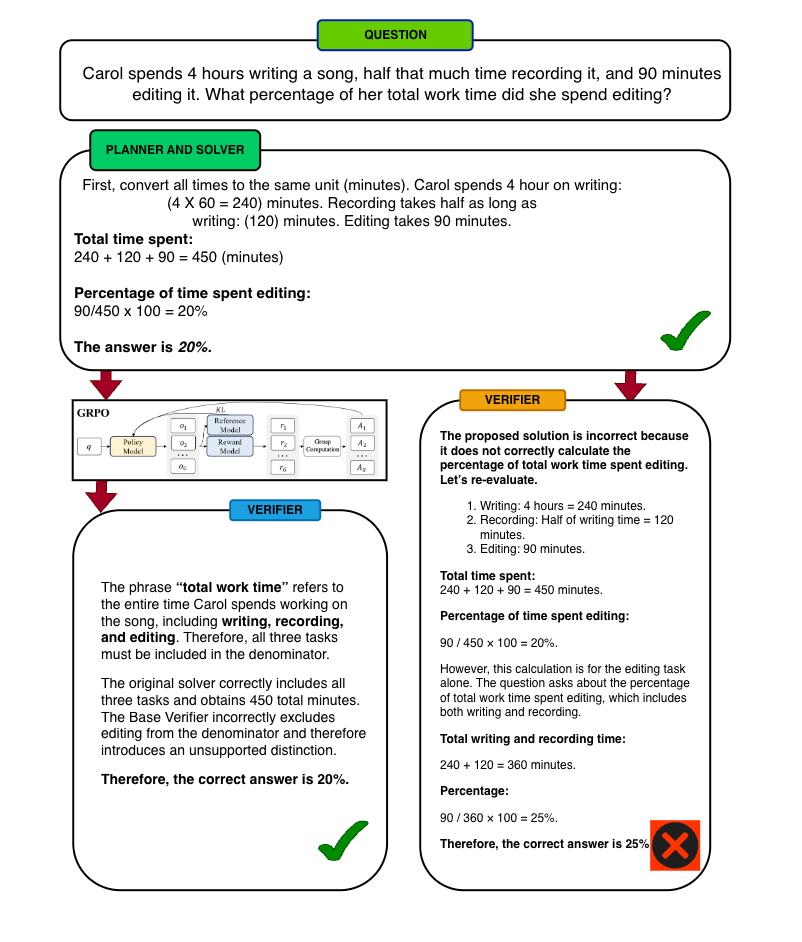
\includegraphics[width=0.65\linewidth]{figs/verifier_grpo_example.png}
\caption{Ví dụ cụ thể trên GSM8K: solver giải đúng (20\%), verifier gốc “sửa” thành sai (25\%) --- đúng kiểu phá vùng rủi ro của \S\ref{sec:termL}; verifier sau GRPO giữ nguyên đáp án đúng, nhưng đạt được điều đó chủ yếu bằng cách can thiệp ít đi, không phải kiểm tra tốt hơn. Hình tái sử dụng từ báo cáo khối Shapley của nhóm.}
\label{fig:grpoexample}
\end{figure}

Nhóm đã thử bảy phương pháp huấn luyện/tối ưu vai trò (Bảng~\ref{tab:rl}). Không phương pháp nào đạt chuẩn dự án (hiệu ứng vượt ngưỡng và 5/5 fold cùng dấu) trên tập lạ, và mỗi thất bại đều truy được về việc model tìm ra lối tắt của hàm mục tiêu thay vì học năng lực đích.

\emph{thứ nhất}: GRPO verifier với thưởng $+1$ cho sửa đúng, $-1$ cho phá, $0$ cho im lặng. Sau huấn luyện, precision tăng từ $0{,}70$--$0{,}90$ lên $1{,}00$ (5/5 fold), nhưng \texttt{V\_gain} giảm từ $+6{,}8$ xuống $+4{,}4$ điểm, và số lần can thiệp giảm từ $20{,}2$ còn $8{,}4$ trên 100 câu. Lối tắt được xác định là “im lặng miễn phí”: precision hoàn hảo đạt được nhờ model nói ít đi một nửa.


\emph{thứ hai}: GRPO theo đáp án cuối (vá lỗ im lặng) đạt $+1{,}8$ điểm, thấp hơn ngưỡng $+2{,}0$ đã đăng ký trước. Lối tắt là nhại solver: trung vị độ dài đầu ra giảm từ $480$ xuống $19$ ký tự, tỷ lệ đồng ý khi solver sai tăng từ $0{,}50$ lên $0{,}64$.

\emph{thứ ba}: GRPO + bất đối xứng thông tin (solver 0,5B, verifier 1,5B; tiền đăng ký, đủ nhánh $I$) đo đồng thời hai mốc: so với model yếu cho $+17{,}0$ điểm (5/5 fold dương); so với chính model kiểm khi tự giải cho $-10{,}4$ điểm (5/5 fold âm). RL chỉ gỡ được 38\% thiệt hại tiếp xúc; 54\% bài hỏng sinh ra đáp án thứ ba không theo ai.

\emph{thứ tư}: ORPO aggregator (học từ cặp ưa thích) đạt $+3{,}3$ điểm trên MATH (3/5 fold, dưới mức dao động nền) và $-2{,}7$ điểm trên GSM8K chéo task. Lối tắt là khuếch đại tật chép ứng viên cuối (từ $0{,}71$ lên $0{,}81$) và học “tự giải lại” thay vì chọn.

\emph{thứ năm}: Credit-RL (thưởng bằng phần đóng góp Shapley biên) không giúp vai trò nào cải thiện theo chuẩn 5/5 fold. Planner sập về plan rỗng trong 200/200 câu; verifier có 23 lần sửa và 24 lần phá.

\emph{thứ sáu}: Credit-RL giai đoạn 2 (thiết kế chống lối tắt) cho V-COND $+3{,}0$ điểm (4/5 fold dương) trên GSM8K, là biến thể dương duy nhất, nhưng không chuyển miền: trên MATH cho $-7{,}0$ điểm (5/5 fold âm).

\emph{thứ bảy}: MAPoRL đồng huấn luyện S/V/A cho kết quả không đổi ($0{,}690 \to 0{,}690$), vì aggregator bị nghẽn suốt quá trình huấn luyện.

\begin{table}[t]\centering\small
\begin{tabular}{p{0.29\linewidth}p{0.33\linewidth}p{0.29\linewidth}}\toprule
Phương pháp & Kết quả chính & Lối tắt tìm thấy\\\midrule
GRPO verifier; thưởng $+1$ sửa / $-1$ phá / $0$ im lặng &
precision $0{,}70$--$0{,}90 \to 1{,}00$ (5/5 fold) \emph{nhưng} \texttt{V\_gain}
$+6{,}8 \to +4{,}4$ điểm; can thiệp $20{,}2 \to 8{,}4$/100 câu &
``im lặng miễn phí'': precision hoàn hảo nhờ nói ít đi một nửa\\[2pt]
GRPO; thưởng theo đáp án cuối (vá lỗ im lặng) &
$+1{,}8$ điểm $<$ ngưỡng $+2{,}0$ đã khoá trước &
nhại solver: trung vị đầu ra $480 \to 19$ ký tự; đồng ý-khi-solver-sai $0{,}50 \to 0{,}64$\\[2pt]
GRPO + bất đối xứng thông tin (solver 0,5B, verifier 1,5B; tiền đăng ký, đủ nhánh $I$) &
so model yếu: $+17{,}0$ điểm (5/5 dương); so chính model kiểm tự giải: $\mathbf{-10{,}4}$
điểm (5/5 \emph{âm}) &
RL chỉ gỡ 38\% thiệt hại tiếp xúc; 54\% bài hỏng ra đáp án \emph{thứ ba} không theo ai\\[2pt]
ORPO aggregator (học từ cặp ưa thích) &
MATH $+3{,}3$ (3/5 fold, dưới mức dao động nền); GSM8K chéo task $-2{,}7$ &
khuếch đại tật chép-ứng-viên-cuối ($0{,}71 \to 0{,}81$); học ``tự giải lại'' thay vì chọn\\[2pt]
Credit-RL (thưởng $=$ phần đóng góp Shapley biên) &
0/4 vai trò cải thiện theo chuẩn 5/5 fold &
planner sập về plan \emph{rỗng} 200/200 câu; verifier 23 sửa / 24 phá\\[2pt]
Credit-RL giai đoạn 2 (thiết kế chống lối tắt) &
V-COND $+3{,}0$ (4/5) trên GSM8K --- biến thể dương duy nhất &
không chuyển miền: trên MATH $-7{,}0$ (5/5 âm)\\[2pt]
MAPoRL đồng huấn luyện S/V/A &
$0{,}690 \to 0{,}690$ ($+0{,}000$) &
aggregator nghẽn suốt quá trình huấn luyện\\\bottomrule
\end{tabular}
\caption{Bảy phương pháp huấn luyện vai trò (mỗi phương pháp có tiền đăng ký hoặc cổng hiệu lực;
chi tiết và đính chính từng lần chạy trong \texttt{docs/}). Phương pháp thứ tám ---
bộ phân loại supervised --- đã ở Bảng~\ref{tab:clf}.}
\label{tab:rl}
\end{table}

Đáng chú ý nhất là thí nghiệm bất đối xứng thông tin (phương pháp thứ ba), khi đo được đồng thời hai mốc trên cùng một lần chạy. So với model yếu, hiệu ứng là $+17{,}0$ điểm (5/5 fold dương); so với chính model kiểm khi không xem bài, hiệu ứng là $-10{,}4$ điểm (5/5 fold âm). Đây là bản tái lập bằng huấn luyện của nghịch lý mốc so sánh (\S\ref{sec:synthesis}): RL thu hẹp thiệt hại tiếp xúc (gỡ 38\%) nhưng không đảo được dấu của $\dhonest$. Kết luận chung của toàn bộ các phương pháp nối thẳng vào \S\ref{sec:kappa}: khi tín hiệu thưởng cũng chỉ là một tín hiệu học được, quá trình tối ưu hoá tìm đến lối tắt của tín hiệu nhanh hơn tìm đến năng lực kiểm tra thực sự.
